% !TEX program = xelatex

%%%%%%%%%%%%%%%%%%%%%%%%%%%%%%%%%%%%%%%%%
% Thin Sectioned Essay
% LaTeX Template
% Version 1.0 (3/8/13)
%
% This template has been downloaded from:
% http://www.LaTeXTemplates.com
%
% Original Author:
% Nicolas Diaz (nsdiaz@uc.cl) with extensive modifications by:
% Vel (vel@latextemplates.com)
%
% License:
% CC BY-NC-SA 3.0 (http://creativecommons.org/licenses/by-nc-sa/3.0/)
%
%%%%%%%%%%%%%%%%%%%%%%%%%%%%%%%%%%%%%%%%%

%----------------------------------------------------------------------------------------
%	PACKAGES AND OTHER DOCUMENT CONFIGURATIONS
%----------------------------------------------------------------------------------------

\documentclass[a4paper, 11pt]{article} % Font size (can be 10pt, 11pt or 12pt) and paper size (remove a4paper for US letter paper)
\usepackage[table]{xcolor}
\usepackage{fontspec}
\definecolor{keycolor}{RGB}{172, 42, 42}
\definecolor{mbleu}{RGB}{64,96,127}
\definecolor{vimvert}{RGB}{46, 139, 87}
\usepackage{hyperref}

% \setmainfont{Avenir Next}
% \setsansfont{Avenir Next}

\usepackage{xeCJK}

\usepackage{geometry}
\geometry{left=2.54cm, top=2.54cm, right=2.54cm, bottom=2.54cm}
\usepackage{subcaption}
\usepackage{tikz}
\usetikzlibrary{tikzmark}
\usepackage{listings}
\usepackage{color}
\usepackage{forest}
\usepackage{float}
\usepackage{makecell}
\usepackage[binary-units]{siunitx}

\lstset{
basicstyle=\small,%
escapeinside=``,%
keywordstyle=\color{blue} \bfseries,% \underbar,%
identifierstyle={},%
commentstyle=\color{blue},%
stringstyle=\ttfamily,%
%labelstyle=\tiny,%
extendedchars=false,%
linewidth=\textwidth,%
numbers=left,%
numberstyle=\tiny \color{blue},%
frame=trbl%
}
 
\newcounter{code}
\lstnewenvironment{code}[3][C++]%
  {%
    \renewcommand\lstlistingname{代码}
    \lstset{% frame=tb,
    language=#1,
    caption=#2,
    label=#3
    }
  }{}

% \usepackage{fancyhdr}
% \usepackage{lastpage}
% \pagestyle{fancy}
% \fancyhf{}
% \fancyfoot[R]{第 \thepage 页,共 \pageref{LastPage} 页}
% % \fancyfoot[C]{\thepage/\pageref{LastPage}}
% \renewcommand{\headrulewidth}{0pt} 
% \renewcommand{\footrulewidth}{0.4pt} 

% \usepackage[protrusion=true,expansion=true]{microtype} % Better typography
\usepackage{graphicx} % Required for including pictures
\usepackage{wrapfig} % Allows in-line images
\usepackage{newfloat}
\usepackage{amsmath}
\usepackage{multirow}

\usepackage{mathpazo} % Use the Palatino font
\usepackage[T1]{fontenc} % Required for accented characters
\linespread{1.2} % Change line spacing here, Palatino benefits from a slight increase by default
% \setlength{\parskip}{0.2em}

\usepackage{indentfirst}
\setlength{\parindent}{2em}

\makeatletter
\renewcommand\@biblabel[1]{\textbf{#1.}} % Change the square brackets for each bibliography item from '[1]' to '1.'
\renewcommand{\@listI}{\itemsep=0pt} % Reduce the space between items in the itemize and enumerate environments and the bibliography

\renewcommand{\maketitle}{ % Customize the title - do not edit title and author name here, see the TITLE block below
\begin{center} % Right align
{\LARGE\@title} % Increase the font size of the title

\large{\@subtitle}

\vspace{1em} % Some vertical space between the title and author name

{\large\@author} % Author name
% \\\@date % Date

% \vspace{1.5em} % Some vertical space between the author block and abstract
\end{center}
}

\renewcommand{\figurename}{图}
\renewcommand{\tablename}{表}

%----------------------------------------------------------------------------------------
%	TITLE
%----------------------------------------------------------------------------------------

\title{\textbf{操作系统实验项目}\\ % Title
} % Subtitle
\newcommand\@subtitle{接管裸机的控制权实验报告}

\author{郑戈涵\quad 17338233\quad 931252924@qq.com} % Institution

\date{2020年4月22日} % Date


%----------------------------------------------------------------------------------------

\begin{document}

\maketitle % Print the title section

%----------------------------------------------------------------------------------------
%	ABSTRACT AND KEYWORDS
%----------------------------------------------------------------------------------------

\renewcommand{\abstractname}{摘要} % Uncomment to change the name of the abstract to something else

\begin{abstract}
  本次实验总共完成两个任务:搭建和应用实验环境和接管裸机的控制权
\end{abstract}

% \hspace*{3,6mm}\texttt{Keywords:} lorem , ipsum , dolor , sit amet , lectus % Keywords

\vspace{1em} % Some vertical space between the abstract and first section

\setcounter{tocdepth}{2}
\renewcommand{\contentsname}{目录}
\tableofcontents

% \vspace{2em} % Some vertical space between the abstract and first section

\pagebreak

\section{实验目的}

% 问题、方法、实验目的、意义
\begin{enumerate}
  \item 了解原型操作系统设计实验教学方法与要求 
  \item 了解计算机硬件系统开机引导方法与过程 
  \item 掌握操作系统的引导程序设计方法与开发工具 
  \item 复习加强汇编语言程序设计能力 
\end{enumerate}


\section{实验要求}

\begin{enumerate}
  \item 知道原型操作系统设计实验的两条线路和前6个实验项目的差别 
  \item 掌握PC电脑的开机引导方法与过程的步骤 
  \item 在自己的电脑上安装配置引导程序设计的开发工具与环境 
  \item 参考样版汇编程序,完成在PC虚拟机上设计一个引导程序的完整工作。 
  \item 编写实验报告,描述实验工作的过程和必要的细节,以证实实验工作的真实性 
\end{enumerate}

\section{实验内容}

% 输入、输出形式,使用的数据结构,算法的描述,算法正确性说明,算法分析,算法实现所需变量,没有代码
\subsection{搭建和应用实验环境}
虚拟机安装,生成一个基本配置的虚拟机XXXPC和多个1.44MB容量的虚拟软盘,将其中一个虚拟软盘用DOS格式化为DOS引导盘,用WinHex工具将其中一个虚拟软盘的首扇区填满你的个人信息。

\subsection{接管裸机的控制权}

设计IBM\_PC的一个引导扇区程序,程序功能是:用字符‘A’从屏幕左边某行位置45度角下斜射出,保持一个可观察的适当速度直线运动,碰到屏幕的边后产生反射,改变方向运动,如此类推,不断运动

\section{实验原理}
\subsection{主引导扇区}
读取的主引导扇区数据有 512 字节,ROM-BIOS 程序将它加载到逻辑地址 0x0000:0x7c00
处,也就是物理地址 0x07c00 处,然后判断它是否有效。
一个有效的主引导扇区,其最后两字节应当是 0x55 和 0xAA。ROM-BIOS 程序首先检测这两
个标志,如果主引导扇区有效,则以一个段间转移指令 jmp 0x0000:0x7c00 跳到那里继续执行 \cite{assembly}
\subsection{字符显示原理}
由于历史的原因,所有在个人计算机上使用的显卡,在加电自检之后都会把自己初始化到
80×25 的文本模式。在这种模式下,屏幕上可以显示 25 行,每行 80 个字符,每屏总共 2000 个
字符的代码存放到显存里,第 1 个代码对应着屏幕左上角第 1 个字符,第 2 个代码对应着屏幕左上角第 2 个字符,后面的依次类推。
屏幕上的每个字符对应着显存中的两个连续字节,前一个是字符的 ASCII 代码,后面是字符的
显示属性,包括字符颜色(前景色)和底色(背景色)。\cite{assembly}

\section{实验过程}
\subsection{编写汇编代码}
代码参考了老师提供的\textit{stoneN.asm},程序有两个要求,一是字符动态显示,二是名字静态显示。
\subsubsection{字符动态显示}
为了让字符能够碰撞屏幕,字符的运动状态需要被记住,总共四种,左上,左下,右上,右下,每种状态遇到屏幕的四个边界都有对应的反应。为了使字符持续运动,运动过程需要在一个死循环中。
代码开始先初始化段寄存器,然后进入循环,循环开始先延迟一段时间,用于控制画框的速度。然后设置初始运动状态(右下)和位置(7,0),用状态和预设定好的状态对应数字依次比较,并跳到不同状态对应的代码执行。
下面以右下为例,右下状态下在遇到右边界和下边界时反弹,\textit{decrement x,y}坐标后需要分别与25,80比较是否到达边界。若到达,跳转到对应的代码执行。跳转到的这部分代码将直接修改坐标和状态。没到则跳转到显示部分\textit{show}的代码执行。
\begin{lstlisting}[language={[x86masm]Assembler}]
DnRt:
	inc word[x]
	inc word[y]
	mov bx,word[x]
	mov ax,25
	sub ax,bx
		jz  dr2ur
	mov bx,word[y]
	mov ax,80
	sub ax,bx	
		jz  dr2dl
	jmp show
\end{lstlisting}
显示部分的代码先将\textit{ax}寄存器清零,并且计算\textit{x,y}对应的显存中的偏移量$$(80*x+y)*2$$,这么计算的理由在原理部分有描述。然后用\textit{ax}寄存器设置属性,我将属性存在数据区,每次设置时取出并加1,即可在每次显示的时候产生不同的效果。最后将属性放入显存\textit{[es:bx]}对应位置中完成显示,一轮循环结束。
\subsubsection{名字静态显示}
静态显示的字符坐标是固定的,将字符属性放入显存中的对应位置就完成了显示。

\subsection{在虚拟机中加载程序}

写好汇编程序后将下述代码保存为run.sh
\begin{code}{生成镜像:run.sh}{code:b-leaf-physical}
nasm main.asm -o main.bin
dd conv=sync if=main.bin of=boot.img bs=1440k count=1  
\end{code}
在命令行中执行即可生成镜像(.img)文件,在VMware中创建新虚拟机并加载改镜像,查看结果。

\section{程序使用说明}
\subsection{实验环境}

\subsubsection{WinHex工具}
WinHex是一个德国软件公司X-Ways所开发的十六进制数据编辑处理程序
\subsubsection{VMware Workstation 15}
VMware Workstation是VMware公司推出的一款桌面虚拟计算软件,具有Windows、Linux 版本。此软件可以提供虚拟机功能,使计算机可以同时运行多个不同操作系统。此次实验中用于运行镜像文件。
\subsubsection{nasm}
Netwide Assembler 是一款基于英特尔 x86 架构的汇编与反汇编工具。在此次实验中用生成二进制文件(.bin)
\subsubsection{Ubuntu 18.04}
本次实验需要制作镜像文件(.img),linux系统提供了dd命令,可以用于将bin文件转换成镜像文件。
% 如何编译和使用程序

\subsection{编译方法}
\subsubsection{系统要求}

本程序要求linux操作系统,需要安装\textit{nasm}。

\subsubsection{编译过程与参数}

在源代码目录下,执行下列代码即可得到镜像文件boot.img。
\begin{code}{生成镜像}{code:b-leaf-physical}
  ./run.sh
\end{code}

\subsection{运行与演示}

在虚拟机软件(此实验中为VMware Workstation)中创建虚拟机,将镜像作为软盘载入,设置随虚拟机启动后启动虚拟机即可。

运行结果如图 \ref{fig:run} 所示。

\begin{figure}[H]
  \centering
   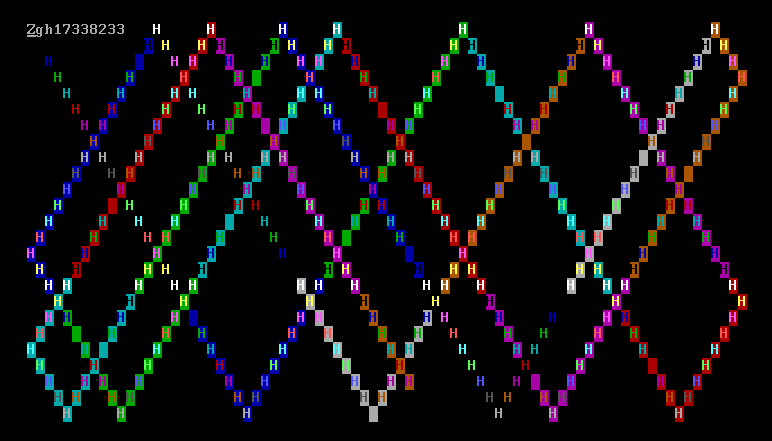
\includegraphics[width=0.8\linewidth]{run.png}
  \caption{运行过程截图}
  \label{fig:run}
\end{figure}

\section{总结与讨论}

% 特色、问题、教训、改进、收获


\subsection{特色,不足与改进}

本程序通过修改字体属性使得每次字符运动时都会显示出不同的样式。
但是受镜像大小约束,我并没有将全名都显示出来。若要显示,不能将代码放在主引导区,需要利用其它盘块。

\subsection{收获}

通过本次实验,笔者复习了x86汇编,了解到了一些新的关键字的用法,比如\textit{equ},\textit{inc},\textit{dec}等。
也对操作系统的启动过程,字符的显示机制有了更深入的了解。同时,在本报告的编写过程中,笔者也练习了利用 \LaTeX 编写文档的能力。\cite{lamport94, cite}

\subsection{感想}

作为操作系统的第一个实验,虽然任务的要求比较少,笔者但是第一次使用这些工具时有较强的生疏感,使用时也遇到了不少麻烦,
比如dd命令在\textit{linux}环境下自带,然而在\textit{windows}环境下需要寻找替代品,这也是笔者后来改用\textit{linux}系统完成编译工作的原因。
并且笔者对\textit{x86}汇编不如\textit{mips}熟悉,而老师提供的代码也有一点小错误,导致运行时看不到结果。
因此笔者花了一些时间复习了x86汇编。关于显存的问题,笔者查看ppt也没有完全理解,但是老师推荐的《x86 汇编语言:从实模式到保护模式》
对这次实验的原理提供了详细的解释,对笔者有很大的帮助。所以这次实验总体上遇到的问题不算多,与同学讨论也能基本得到答案,还是比较顺利的。

\begin{thebibliography}{99}

	\bibitem{lamport94}
    Leslie Lamport,
    \textit{\LaTeX: a document preparation system},
    Addison Wesley, Massachusetts,
    2nd edition,
    1994.
  \bibitem{assembly}
    李忠,王晓波,余洁,
    \textit{x86 汇编语言:从实模式到保护模式},
		电子工业出版社,
    2012.
  \bibitem{cite}
    Contributors to Wikibooks,
    \textit{LaTeX Bibliography Management.}
    Wikibooks,
    2019., \\
    en.wikibooks.org/wiki/LaTeX/Bibliography\_Management.


\end{thebibliography}

%----------------------------------------------------------------------------------------

\end{document}